% !TeX program = pdflatex
\documentclass[tikz,border=8pt]{standalone}
\usepackage{tikz}\usetikzlibrary{calc}
\definecolor{FigureBlue}{HTML}{2563EB}
\begin{document}
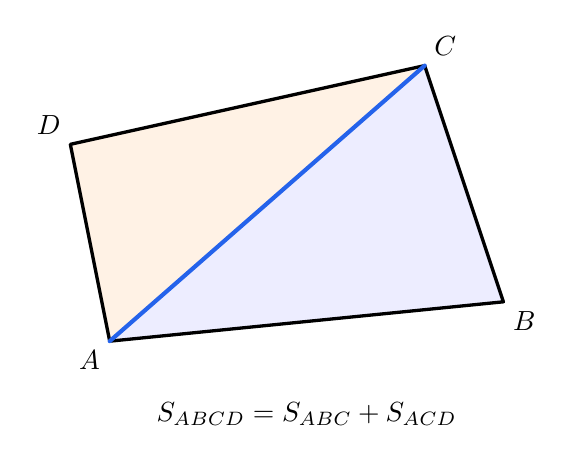
\begin{tikzpicture}[line cap=round,line join=round]
  \coordinate (A) at (0,0); \coordinate (B) at (5,.5); \coordinate (C) at (4,3.5); \coordinate (D) at (-.5,2.5);
  \fill[blue!7] (A)--(B)--(C)--cycle; \fill[orange!10] (A)--(C)--(D)--cycle;
  \draw[line width=1.2pt] (A)--(B)--(C)--(D)--cycle; \draw[FigureBlue,line width=1.5pt] (A)--(C);
  \node[below left] at (A) {$A$}; \node[below right] at (B) {$B$}; \node[above right] at (C) {$C$}; \node[above left] at (D) {$D$};
  \node[below=9mm] at ($(A)!.5!(B)$) {$S_{ABCD}=S_{ABC}+S_{ACD}$};
\end{tikzpicture}
\end{document}
